\documentclass{acm_proc_article-sp}
\begin{document}

\title{particle Generalized FEM
-basic idea and selected examples}
%\subtitle{[Extended Abstract]

\numberofauthors{1} %  in this sample file, there are a *total*
% of EIGHT authors. SIX appear on the 'first-page' (for formatting
% reasons) and the remaining two appear in the \additionalauthors section.
%
\author{
% 1st. author
\alignauthor
Rong Tian\\
       \affaddr{Institute of Computing Technology, Chinese Academy of Sciences,}\\
       \affaddr{Kexueyuan Nanlu 6, Haidian, Beijing 100190, China}\\
       \email{rongtian@ncic.ac.cn}
}
\date{30 June 2013}

\maketitle

\begin{abstract}
A 'head-to-toe', naturally parallelizable finite element approach is proposed. The method is designed to be scalable with an unstructured mesh of any complicated geometry and any large size.
In large deformation analysis the method also offers strong mesh distortion tolerance. The
numerical performance of the method is verified and demonstrated through numerical examples in 3D.
\end{abstract}

\terms{Theory}

\keywords{particle generalized finite element method, partition of unity, parallel finite element method, mesh distortion.} % NOT required for Proceedings

\section{Introduction}
Powered by petaflops (1015 flop operations per second) supercomputers, numerical simulation steps into a completely new era; a parallel FE code at this scale is expected to use processor cores of order of hundreds of thousands. The above mentioned conventional parallel FE procedure would be hampered by its poor scalability in pre- and post-processing (Figure 1(a)). As a typical example, unstructured mesh generation at scale is no longer a routine task and already a defacto bottleneck of scalability. Visualization and IO of data in tera- and petabytes also would not be feasible without resorting to parallel techniques\cite{rongtian:method}.
In this paper, a particle generalized FEM is proposed with two purposes: (a) easy implementation at scale; (b) high tolerance to mesh distortion. Figure 1(b) is used to illustrate the proposed method.Compared with the conventional parallel FEM, the proposed method is expected to overcome the serious bottleneck of unstructured mesh generation and to be embarrassing parallel in the pre and the post processes.

\section{The method}
\subsection{Basic idea}
Let $\bigcup M_i^{geo}$ denote an assembly of meshes $M_i^{geo}$ that are non-overlapping, non-conforming, and completely independent meshes. The mesh assembly forms a non-overlapping and seamless
decomposition of $\Omega$ , and is called \emph{geometric mesh} or \emph{physical mesh}, labeled by superscript "geo". Let $M^{math}$ = {\emph{cell}($h_x \times h_y \times h_z$)} be a Cartesian structured grid called \emph{math grid} that covers $\Omega$ and it is independent of $\Omega$. $h_x, h_y, h_z$ are respectively the math cell size in $x, y, z$ coordinate direction. The vertex of the geometric mesh and the math grid is called, respectively, \emph{physical node and math node}, and the element of each set of mesh is termed, respectively, \emph{geometric/physical element}, and \emph{math cell}.
For the problem of interest, given a strong form of PDEs
\begin{equation}
\begin{cases}
  	   \textbf{A}(\textbf{u})=0; &in  \Omega\\
       \textbf{B}(\textbf{u})=0; &in  \Gamma\\  
\end{cases}
\end{equation}
which are, respectively, the differential equation set to be satisfied in the volume of material, $\Omega$, and on the boundary of the domain, $\Gamma$, a general statement of the Galerkin weighted residual approach is expressed as
\begin{equation}
\int_{\Omega}\textbf{N}^T\textbf{A}(\textbf{Nu})d\Omega + \int_{\Gamma}\textbf{N}^T\textbf{B}(\textbf{Nu})d\Gamma = 0  
\end{equation}
The reason that the pGFEM is called a \emph{particle} method is that the geometric mesh, as it is mainly used for a quadrature purpose, merely appears in form of a Gauss point set during momentum equation solving (but the location and the weight of the Gauss points are still updated by reference to the geometric mesh). As such, during the solving phase of the momentum equations, although we employ two sets of meshes, the geometric mesh is actually really used as a set of points. In addition,the connectivity between a given Gauss point and a math node is not pre-defined but in a runtime/dynamic manner. The particle feature and the dynamic connectivity make the proposed method more like a particle method of the meshfree class.\cite{bramms:babel}
\begin{figure}
\centering
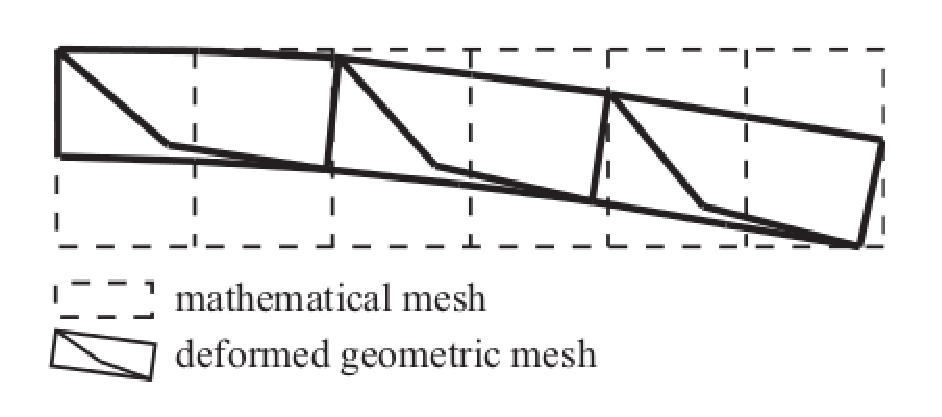
\epsfig{file=figure1.eps, height=1.5in, width=2in}
\caption{A typical pGFEM mesh in large deformation analysis}
\end{figure}

\subsection{Step total Lagrangian formulation}
Let $\textbf{x}^n$ be an intermediate configuration. Assume the material can be mapped one by one between the current configurations $\textbf{x}$ and $\textbf{x}^n$, i.e., there is no cracking and splitting of a material point, we express $\textbf{x}$ with respect to $\textbf{x}^n$ as\cite{Lamport:LaTeX}.
\begin{equation}
\textbf{x}(\textbf{x}^n,t) = \textbf{x}^n + \Delta\textbf{u}(t)
\end{equation}
where $\Delta\textbf{u}(\textbf{t})$ is finite deformation.

\section{Relations with the existing methods}
The pGFEM follows a line of a partition of unity-based generalized FEM (Strouboulis et al. (2001)) and is designed to combine together with the major advantage of the Material Point Method (Sulsky et al. (1994), Zhang et al. (2006)) in avoiding mesh distortion in tracing large deformation and deformation discontinuity. The same as the MPM, the pGFEM solves the momentum equation on an independent and regular math grid. The MPM is an explicit method and hence the data projection, such as mass and momentum etc, between the material points and the background mesh has to be done every single time step.\cite{clark:pct} The pGFEM is designed as an implicit method and the step total Lagrangian formulation is used to avoid frequent data projection between two meshes. If deformation is moderately large and continuous, then $\textbf{x}^n$ is never necessarily updated and the pGFEM becomes a total Lagrangian method.

\section{Selected examples}
The test is carried out in a nonlinear large deformation setup of the cantilever problem in Figure 3. The material is taken as a compressible Neo-Hooken material. The point preconditioned conjugate gradient method is used to solve the system equation. Line search is used to search the solution of Newton iterations. The load at the free end is applied evenly in 10 steps. To make the test general, the intermediate configuration $\textbf{x}^n$ is updated every load step so that the math grid aligns the outer boundary of the cantilever only at the first load step and from the first step on the math grid misaligns with the geometric mesh like that in Figure 4. Noted is that this is the worst scenario in practical use and it is used on purpose to test the method's robustness.\cite{herlihy:methodology}

\begin{figure}
\centering
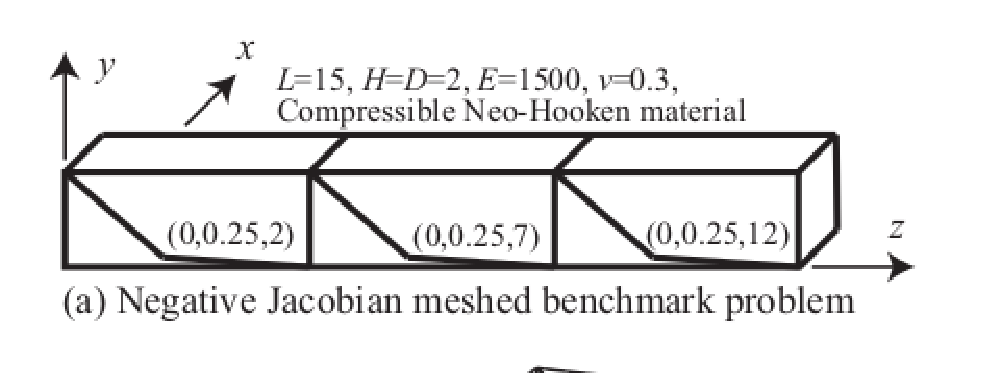
\epsfig{file=figure2.eps, height=1.5in, width=2.5in}
\caption{Negative Jacobian meshed benchmark problem}
\end{figure}

\begin{tabular}{|c|c|c|c|}\hline
{\emph MergeSort} & 0.05s    & 0.62s   & 7.07s  \\\hline
{\emph QuickSort} & 0.03s    & 0.40s   & 4.75s  \\\hline
{\emph M\_QuickSort} & 0.04s    & 0.42s   & 5.04s  \\\hline
{\emph MergeSort\_Stack} & 0.06s    & 0.68s   & 7.71s  \\\hline
{\emph QuickSort\_Stack} & 0.04s    & 0.50s   & 5.72s  \\\hline
{\emph M\_QuickSort\_Stack} & 0.04s    & 0.48s   & 5.47s  \\\hline
\end{tabular}\\


\section{Concluding remarks}
A particle generalized FEM has been developed, motivated by the potential scalability issue of parallel FE simulation at extreme scale. The pGFEM is designed to be naturally parallelizable. The method has a potential in overcoming the difficulties in pre- and post processes at scale, in particular making unstructured mesh generation easy. Analytical and numerical studies showed the method is also not sensitive to mesh distortion.\cite{salas:calculus}


%ACKNOWLEDGMENTS are optional
\section{Acknowledgments}
Without Qingxu, nothing will be much worth doing.

%
% The following two commands are all you need in the
% initial runs of your .tex file to
% produce the bibliography for the citations in your paper.
\bibliographystyle{abbrv}
\bibliography{sigproc}  % sigproc.bib is the name of the Bibliography in this case
% You must have a proper ".bib" file
%  and remember to run:
% latex bibtex latex latex
% to resolve all reference

\end{document}
